\chapter{Analysis of results}
\label{ch:Results}
\ifpdf
\graphicspath{{Chapter5/Chapter5Figures/}}
\fi

This chapter discusses the accuracy of the test grading system. In the first two sections of this chapter, the basic and complete system are compared using the same datasets. The first test grading system includes only image processing techniques described in Chapter \ref{ch:ImageProcessing}. The second system contains the complete project software with all the machine learning techniques described in Chapter \ref{ch:MachineLearning}.

Each system is assessed using two categories. The first category describes all the tests the system transferred to the user for manual marking. The reason for this is that the system calculated a certainty level below a specific threshold for that particular test. In this category the tests are send to a clash list. After all the tests are graded, the system displays an interface with values it estimated the student wrote down. An additional image of the test is also displayed. The user is then tasked with looking through each of the clash list tests, using the interface, to see if any tests is graded incorrectly by the system. This process is normally fast, as the system has a high accuracy in predicting the answers correctly. In the last category, all the answers that the system decided to grade automatically, but identified incorrectly, is described.

\section{Results of 25 test cases}

In this section the results of grading 25 hand picked tests are compared between the two systems. Among the 25 tests, there are different categories that evaluate different aspects and limitations on both systems. The categories and the number of tests for the particular category, are listed in Table \ref{tbl:25Tests}.

\begin{table}
\caption{Description of 25 evaluation tests.} \label{tbl:25Tests}
  \centering
\begin{tabular}{|p{6cm}|p{4cm}|}
\hline
\textbf{Description of test type}&\textbf{Number of tests}\\
\hline
Test with crossed-out answers&7\\
\hline
Test with lightly coloured entries or partially coloured-in entries&4\\
\hline
Test with negative signed answers&1 (also included under other categories)\\
\hline
Test with no bubbles and only characters filled in for a specific entry field &5\\
\hline
Test with no characters filled in and only bubbles for a specific entry field&2\\
\hline
Test with data filled in correctly&2\\
\hline
Page with no template on it (Possible scanned upside down)&2\\
\hline
Page with rotated template inside image&2\\
\hline
\end{tabular} 
\end{table}

These tests are specifically chosen, because combined, they approximates all the types of tests the system have to assess. Most of the tests are extreme cases of what students have filled in on test forms. These tests provide a good benchmark to determine how well each system performs in challenging situations.

\subsection{Basic system}
Using the basic system, an average time evaluating each test is calculated to be 0.305 seconds on the grading computer. An overall grading accuracy of 84.6\% was recorded for this system.

\begin{figure}
  \centering
  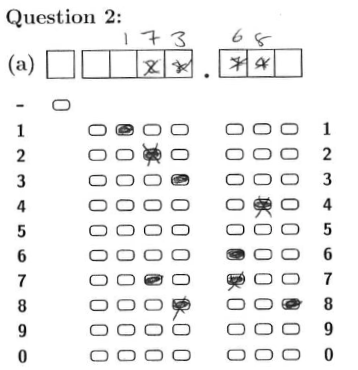
\includegraphics[width=8cm]{crossClash}\\
  \caption{Image showing answer with crossed-out answers that the system misinterpreted.}
  \label{fig:crossClash}
\end{figure}

\subsubsection{Clash list}
A total of 6 out of the 25 tests were reported as clashes. The two images without a template were reported in the clash list. Furthermore, 1 test which only has the student number written in characters with no bubble information was also reported to the list. The other 3 clashes were reported due to the crossed-out bubbles being interpreted as still filled in, causing the system to think that two answer bubbles were filled in. An example of this is shown in Figure \ref{fig:crossClash}.

\subsubsection{Incorrect automatic graded results}

There where 4 tests that where graded automatically, but incorrectly. All of these tests had only character information in at least one of the answers. An example of this can be seen in Figure \ref{fig:OnlyCharacters}.

\begin{figure}
  \centering
  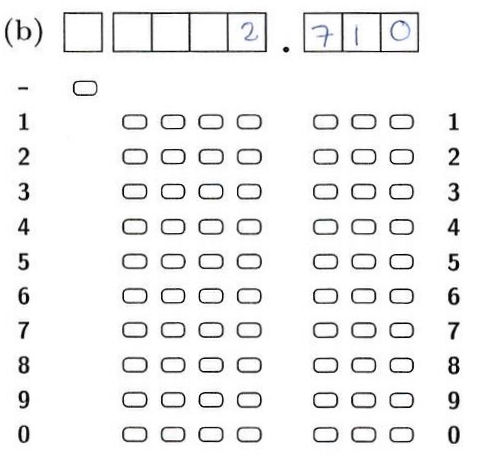
\includegraphics[width=8cm]{OnlyCharacters}\\
  \caption{Filled-in answer with only character information.}
  \label{fig:OnlyCharacters}
\end{figure}

\subsection{Complete system}

Using the complete system, an average time evaluating each test is calculated to be 2.011 seconds. An overall grading accuracy of 100.0\% was recorded for this system.

\subsubsection{Clash list}

A total of 6 out of the 25 test where reported as clashes. The two images with no template in were again reported in the clash list. Two cases was reported to the clash list due to the character recognition determining a crossed-out character as the intended character, but with low certainty. An example of this is shown in Figure \ref{fig:crossedOutCharacter}. One test was reported, because it only had characters in with no bubbles coloured in. Thus, even though the system identified every character correctly, it had a too low percentage confidence in its answer and reported it to the clash list. 

\begin{figure}
  \centering
  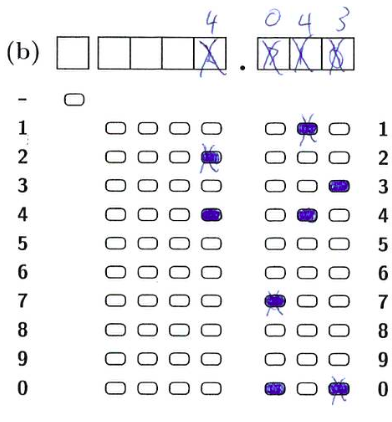
\includegraphics[width=8cm]{crossedOutCharacter}\\
  \caption{Crossed-out character that confused the grading system.}
  \label{fig:crossedOutCharacter}
\end{figure}

\subsubsection{Incorrect automatic graded results}

There were no automatically graded answers that were done incorrectly.

\subsection{Analysis of results}

The systems both had the same number of clash list tests from these 25 images. The complete system took on average 2.011 seconds to grade a test. The student number PGM consumes most of that time, 1.5 seconds, to infer the correct student number. The complete system had no incorrectly automatically graded answers, in contrast to the 4 graded incorrectly using the basic system. A reason to this is attributed to more evidence that are considered in the complete system. Therefore only if the evidence match up will the system be certain enough to accept its answer as the correct one. In the next section the complete system is used to grade a tutorial test written by all the students. 

\section{Grading of tutorial tests}
In this section the complete system is tested on a tutorial written by all the students in the class. The final version of the complete system was used in grading the students' tests. Student feedback was recorded to find tests that were graded incorrectly and used as the grader's results. 

\subsection{Marking statistics}

For these tutorial test an average marking time per test of 2.01 seconds was recorded.

\subsection{Clash list}

There were in total 57 clashes in the 888 tests. These 57 clashes are categorised in Table \ref{tbl:TutClash}.
\begin{table}
  \centering
  \caption{Description and quantity of clashes in the different categories.} \label{tbl:TutClash}
\begin{tabular}{|p{3cm}|p{8cm}|}
\hline
\textbf{Number of tests} & \textbf{Category description}\\
\textbf{in category} &\\
\hline
31&In these tests the system determined the right values, but was unsure about its answer. Some of the cases were when the student number was only filled in the character box. The software always identified the correct student number, but was still uncertain about the answer.\\
\hline
15&In these tests the system could not distinguish between a crossed-out answer and correct answer. This is due to the crossed-out answer being interpreted as a filled in answer.\\
\hline
8&These tests have an answer with only character information in them. The system attempted to identify each answer, but made a mistake in at least one of the digits.\\
\hline
2&These images contained blank papers that did not include test templates.\\
\hline
1&In this test the grid of the test paper could not be found and thus test could not be marked.\\
\hline
\end{tabular}
\end{table}

\subsection{Incorrect automatic graded results}

The students were asked to report any results that were marked incorrectly by the system for this particular test. These results are all the results that the system decided to accept the automatically graded answer, and in doing so, graded the test incorrectly.

Only 1 result was reported where the software automatically marked the answer in an incorrect manner. The correct answer was -95.0 and the system marked the answer as 95.0, as shown in Figure \ref{fig:wrongAns}. There may still be tests that were marked incorrectly, but these tests were not reported. In comparison there were 15 known mistakes made in the first tutorial using the basic system.

\begin{figure}
  \centering
  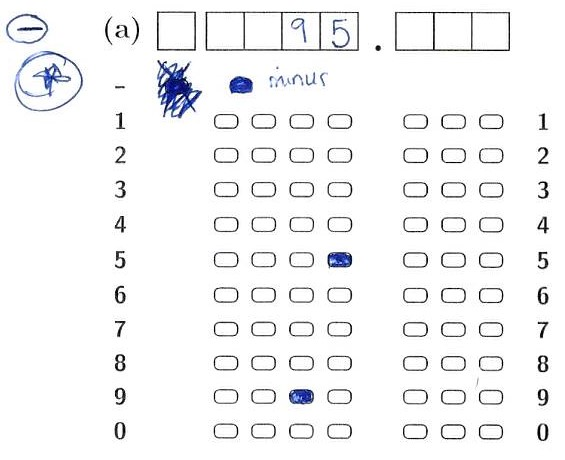
\includegraphics[width=8cm]{wrongResult}\\
  \caption{Incorrectly identified answer as 95.}
  \label{fig:wrongAns}
\end{figure}

For a more detailed description of the results from grading all 4 tutorial tests, refer to Appendix \ref{ap:results}.

\subsection{Conclusion}

In conclusion, it is noted that the complete system, with its machine learning capabilities, reduces the number of tests that the user must mark manually, in comparison with the previous basic system. For this complete system, about 7.5\% of the tests in the tutorial had to be marked manually, due to the system being unsure of the answers. The system does however grade 99.9\% of the tests correctly, when the system decides to grade them automatically. The reason for this can be attributed to the fact that the system correlates two pieces of evidence to predict the correct answer. Thus, both the character and bubble information had to be interpreted incorrectly for the system to automatically grade an answer incorrectly. 

The system could grade 92.5\% of all the test correctly and automatically. From the remaining 7.5\% only 1 test or 0.1\% of the tests was found to be graded incorrectly and the other 7.4\% of the tests were sent to a clash list. The system classified most of the clash list tests correctly. If the clash list threshold level of the system is set to 0 the system could possibly have graded 97.1\% of the tests correctly.

